\documentclass[conference]{IEEEtran}
\usepackage{cite}
\usepackage{amsmath,amssymb,amsfonts}
\usepackage{algorithmic}
\usepackage{graphicx}
\usepackage{textcomp}
\usepackage{xcolor}
\usepackage{comment}
\usepackage{circuitikz}
\usepackage{float}
\usepackage{stfloats}

\def\BibTeX{{\rm B\kern-.05em{\sc i\kern-.025em b}\kern-.08em
    T\kern-.1667em\lower.7ex\hbox{E}\kern-.125emX}}
\begin{document}

\title{Dying Light: Fluorescence Lifetime Analysis\\
}

\author{\IEEEauthorblockN{Samir Afsary}
\IEEEauthorblockA{\textit{Electrical and Systems Engineering} \\
\textit{Washington University in St. Louis}\\
St. Louis, MO \\
a.samir@wustl.edu}
\and
\IEEEauthorblockN{Ahmad Hamzeh}
\IEEEauthorblockA{\textit{Computer Science and Engineering} \\
\textit{Washington University in St. Louis}\\
St. Louis, MO \\
a.hamzeh@wustl.edu}
\and
\IEEEauthorblockN{Alex Ge}
\IEEEauthorblockA{\textit{Electrical and Systems Engineering} \\
\textit{Washington University in St. Louis}\\
St. Louis, MO \\
age@wustl.edu}
}

\maketitle

\begin{abstract}
This paper presents an analysis of fluorescence
lifetime imaging microscopy (FLIM) through three interconnected tasks.
In Task~1 the full time-domain detection of a fluorescence system with
a sufficiently fast detector is modeled from pulsed excitation to 
ditization with an analog-to-digital converter (ADC). Then the fluoorescence frequency response
is verified numerically against the theoretical frequency response of a
single-exponential decay. We then analyze the impact of different
detector impulse response functions (IRFs) on the digitized output 
signal. In Task~2, we demonstrate that direct 100\,kHz sampling of an
80\,MHz fluorescence signal is impossible due to aliasing, then show
that heterodyne mixing to a 1\,kHz intermediate frequency recovers
the original phase shift and modulation depth, yielding an estimated
lifetime of $\tau \approx 1\,\text{ns}$ from both observables.
In Task~3, phasor analysis is derived analytically and applied
pixel-by-pixel to a $512\times512$ TCSPC dataset of NAD(P)H in breast
cancer cells, producing a spatially-resolved lifetime image and a phasor
plot that separates free NAD(P)H ($\tau \lesssim 0.5\,\text{ns}$) from
protein-bound NAD(P)H ($\tau \sim 1$--$3\,\text{ns}$), reflecting the
metabolic heterogeneity of the cell population.
\end{abstract}

\section{Background}

Natural phenomena are often quantized and analyzed through the use of
systems and other mathematical models: the modeling of fluorescence is a
compelling example of such modeling.
Although light is an inherently complex electromagnetic phenomenon, its
behaviors can be modeled using frameworks discussed in our studies of
signals and systems.
Specifically, excitations of photons can be represented by impulses, and
a general system for studying fluorescence lifetime imaging microscopy
(FLIM) is born from a few continuous-time convolutions and
multiplications.
Through this perspective, fluorescence is not only observable but
analytically solvable, allowing techniques from linear time-invariant
system theory to be applied directly to real physical processes.

In the fluorescence process, a fluorophore absorbs optical energy from
an excitation source $x(t)$, exciting an electron to a higher energy
state.
After a brief delay, a photon of slightly lower energy is emitted as the
electron relaxes.
The probability density of this delay follows an exponential decay, so
the fluorescence impulse response function (IRF) is:

\begin{equation}
    h_f(t) = e^{-t/\tau}\,u(t),
    \label{eq:hf}
\end{equation}

where $\tau$ is the fluorescence lifetime and $u(t)$ is the unit step.
The lifetime $\tau$ encodes information about the fluorophore's
nanoscale environment---local temperature, pH, ion concentration, and
protein interactions---and typically falls in the picosecond-to-nanosecond
range~\cite{Datta2020}.
Fluorescence lifetime imaging microscopy (FLIM) measures $\tau$ at
every pixel of a field of view, producing a spatially-resolved map of
biochemical state.

The emitted fluorescence $f(t)$ is collected by a photomultiplier
tube (PMT) with its own impulse response $h_d(t)$, That is then sampled by an ADC.
Depending on the available hardware, lifetime information can be
extracted from time-domain exponential fitting, frequency-domain phase
and modulation analysis, or the phasor approach explored in this
study~\cite{Gadella1993,Digman2008}.

\section{Methods}
\subsection{Task 1: Fast Time-Domain Detection}
\subsubsection{Time Domain Signal Simulation}

Continuous-time convolution is the mathematical operation used to model the signal processing of the fluorescence system. 
Given two continuous-time signals $x(t)$ and $h(t)$, their convolution is defined as:
\begin{equation}
    y(t) = x(t) * h(t) = \int_{-\infty}^{\infty} x(\tau) h(t - \tau) d\tau
\end{equation}
where the output signal $y(t)$ is the result of convolving the input signal $x(t)$ with the system's impulse response function $h(t)$.
We simulated an ideal fluorescence system as a cascade of LTI systems: an inititial pulsed excitation $x(t)$ convolved with the fluorescence IRF $h_f(t)$,
then convolved with the detector IRF $h_d(t)$, and finally sampled by an ADC $p(t)$.
The fluorescence system was simulated over a 125 ns window in continuous time using a high-resolution time step ($dt = 0.001\,\text{ns}$). 
The pulsed laser excitation was modeled as an impulse train $x(t)$:
\begin{equation}
    x(t) = \sum_{n=-\infty}^{\infty} \delta(t - nT_L)
    \label{eq:xl}
\end{equation}
where $T_L = 12.5\,\text{ns}$ is the pulse repetition period. 
To accurately approximate the continuous-time function $\delta(t)$ in a discrete MATLAB array, the impulses were generated with an amplitude of $1/dt$.
This ensures that the mathematical area under each discrete pulse over one time step evaluates to exactly 1 (i.e., $(1/dt) \times dt = 1$), properly preserving the energy of the theoretical excitation pulse. 

The fluorescence emission $f(t)$ was computed by a convolution of $x(t)$ with the fluorescence IRF $h_f(t)$ from \eqref{eq:hf},
with a fluorescence lifetime of $\tau = 1\,\text{ns}$. In MATLAB, the continuous-time integral was approximated digitally by scaling the discrete convolution by our time step $dt$.


The emitted fluorescence was then convolved with a detector IRF to model the PMT:
\begin{equation}
    h_d(t) = e^{-(t-t_0)^2/\sigma_t^2} \, u(t)
    \label{eq:hd}
\end{equation}
Where $h_d(t)$ is a Gaussian distribution made causal by multiplying by the unit step function $u(t)$ used to model the detector IRF.
The variables $\sigma_t$ and $t_0$ represent the width and time offset of the Gaussian distribution, respectively.
For this ideal system, the width of the Gaussian distribution $\sigma_t$ was set to $0.1$ ns, and the time offset $t_0$ was set to $0.175$ ns.
The convolution produces the detector output $d(t)$. In this section there is no extra processing of the signal, so the continuous system output $y(t)$ is equal to $d(t)$.
Finally, the continuous signal was modeled as being sampled by an ADC. The process is represented by multiplying the continuous signal with an impulse train $p(t)$:
\begin{equation}
    p(t) = \sum_{m=-\infty}^{\infty} \delta(t - mT_S)
    \label{eq:pt}
\end{equation}
where $T_s = 0.2\,\text{ns}$ is the sampling period. This yields the discrete-time digitized output signal $y[n] = y(nT_s)$.

\subsubsection{Frequency Response Verification}

To validate our time-domain convolution model, we derived the theoretical continuous-time frequency response of the fluorescence IRF $h_f(t)$ from \eqref{eq:hf}.
The Fourier transform is evaluated as follows:
$$
    H_f(j\omega) = \int_{0}^{\infty} e^{-t/\tau} e^{-j\omega t} dt = \int_{0}^{\infty} e^{-t\left(\frac{1}{\tau} + j\omega\right)} dt
$$
Evaluating the integral limits yields:
$$
    H_f(j\omega) = \left[ \frac{-1}{\frac{1}{\tau} + j\omega} e^{-t\left(\frac{1}{\tau} + j\omega\right)} \right]_{0}^{\infty} = \frac{1}{\frac{1}{\tau} + j\omega}
$$
Multiplying the numerator and denominator by $\tau$ gives the final expression:
\begin{equation}
    H_f(j\omega) = \frac{\tau}{1 + j\omega\tau}
    \label{eq:Hf}
\end{equation}
The theoretical magnitude and phase of $H_f(j\omega)$ are therefore:
\begin{align}
    |H_f(j\omega)| &= \frac{\tau}{\sqrt{1 + (\omega\tau)^2}}, \label{eq:Hf_mag} \\
    \angle H_f(j\omega) &= -\arctan(\omega\tau). \label{eq:Hf_phase}
\end{align}
We then computed the numerical Fourier transform of the simulated fluorescence signal $f(t)$ using MATLAB's Fast Fourier Transform (FFT).
To circumvent the phase plot periodicity from the discrete nature of a FFT, the $dt$ step was replaced with a finer step $dt_{fine}=dt/100$ for the Fourier transform,
and the plots were zoomed in to the range where the phase wrapping is not apparent.
This is because computers are inherently discrete, and the FFT assumes periodicity in the signal, which can lead to phase wrapping if the frequency resolution is not sufficiently high.

\subsection{Detector IRF Impact Analysis}
To characterize the effect of detection hardware on the measured signal,
the convolution and sampling processes for $y[n]$ were repeated across three different $h_d(t)$:
fast ($\sigma_t = 0.1\,\text{ns}, t_0=0.175\,\text{ns}$), medium ($\sigma_t = 2.5\,\text{ns}, t_0=4\,\text{ns}$), and slow ($\sigma_t = 10\,\text{ns}, t_0=17\,\text{ns}$).



\subsection{Task 2: Heterodyne Detection}



\subsection{Task 3: Phasor Analysis}

\subsubsection{Phasor Component Derivation}
\label{sec:phasor_deriv}

Phasor analysis projects the fluorescence decay onto cosine and sine
basis functions at $\omega_L$, yielding two scalar
coordinates~\cite{Digman2008}:

\begin{align}
    g &= \frac{\displaystyle\int_{\langle T_L \rangle}
               h_f(t)\,\cos(\omega_L t)\,dt}
              {\displaystyle\int_{\langle T_L \rangle}
               h_f(t)\,dt},
    \label{eq:g_def}
    \\[4pt]
    s &= \frac{\displaystyle\int_{\langle T_L \rangle}
               h_f(t)\,\sin(\omega_L t)\,dt}
              {\displaystyle\int_{\langle T_L \rangle}
               h_f(t)\,dt}.
    \label{eq:s_def}
\end{align}

For $h_f(t) = e^{-t/\tau}$ integrated from $0$ to $\infty$
(valid when $T_L \gg \tau$, which holds here since $T_L=12.5\,\text{ns}$
and $\tau=1\,\text{ns}$), the integrals evaluate analytically:

\begin{align}
    g &= \frac{1}{1 + (\omega_L\tau)^2},
    \label{eq:g_analytic} \\[4pt]
    s &= \frac{\omega_L\tau}{1 + (\omega_L\tau)^2}.
    \label{eq:s_analytic}
\end{align}

Together, $g$ and $s$ are the real and imaginary parts of
$H_f(j\omega_L)/\tau = 1/(1+j\omega_L\tau)$, so they encode the same
phase and modulation information as heterodyne detection, but without
requiring a reference channel.
The lifetime is recovered as:

\begin{equation}
    \tau = \frac{s}{\omega_L\,g},
    \label{eq:tau_phasor}
\end{equation}

which is self-consistent:
$\tau = (\omega_L\tau)/[\omega_L\cdot 1] = \tau$. $\checkmark$

\textbf{Physical interpretation.}
$g$ (in-phase) is higher for \emph{shorter} lifetimes; as
$\tau\to 0$, $g\to 1$.
$s$ (quadrature) peaks when $\omega_L\tau = 1$, i.e.,
$\tau = 1/(2\pi f_L) \approx 2\,\text{ns}$ at 80\,MHz; it vanishes
for both very short and very long lifetimes.

\textbf{Universal semicircle.}
All single-exponential $(g,s)$ pairs satisfy
$(g - \tfrac{1}{2})^2 + s^2 = \tfrac{1}{4}$, i.e.\ they lie on a
semicircle of radius $\tfrac{1}{2}$ centered at $(\tfrac{1}{2},0)$.
This follows from $g^2 + s^2 = g$, derived by adding
Eqs.~\eqref{eq:g_analytic}--\eqref{eq:s_analytic} after rearrangement.
Multi-exponential or mixed-species pixels fall \emph{inside} the
semicircle at the intensity-weighted average of each species' coordinates.

\subsubsection{Per-Pixel Implementation for FLIM Data}
For time-domain TCSPC data, the continuous integrals become discrete
sums over the photon-count histogram $h_{x,y}[n]$ at pixel $(x,y)$:

\begin{align}
    g_{x,y} &= \frac{\displaystyle\sum_{n=0}^{N_t-1}
                     h_{x,y}[n]\,\cos(\omega_L t_n)}
                    {\displaystyle\sum_{n=0}^{N_t-1} h_{x,y}[n]},
    \label{eq:g_discrete} \\[4pt]
    s_{x,y} &= \frac{\displaystyle\sum_{n=0}^{N_t-1}
                     h_{x,y}[n]\,\sin(\omega_L t_n)}
                    {\displaystyle\sum_{n=0}^{N_t-1} h_{x,y}[n]},
    \label{eq:s_discrete}
\end{align}

where $t_n = n\,\Delta t$, $\Delta t = 0.128\,\text{ns}$, and
$\omega_L = 2\pi/T_L = 2\pi/12.5\,\text{rad/ns}$.
The MATLAB implementation reshapes the $512\times512\times N_t$ data
cube into an $(N_\text{pix}\times N_t)$ matrix and computes both sums
as single matrix--vector multiplies, avoiding any pixel-by-pixel loop.
Pixels with fewer than 10 detected photons were excluded, and lifetimes
outside $[0,\,6]\,\text{ns}$ were masked as unphysical.

\section{Results}

\subsection{Task 1: Fast Time-Domain Detection}

\subsubsection{Time-Domain Signals}
The simulation of the cascaded systems successfully modeled the fluorescence detection process, as shown in Figure \ref{fig:task1a}.
The initial excitation $x(t)$ acts as a clean impulse train with a $12.5\,\text{ns}$ period.
The resulting emitted fluorescence $f(t)$ demonstrates a repeated sharp single-exponential decay that effectively reaches zero before the subsequent pulse.

Because the baseline detector IRF was highly precise ($\sigma_t = 0.1\,\text{ns}$),
the continuous detector output $d(t)$ and the overall system output $y(t)$ preserved the rapid exponential decay of $f(t)$ with minimal blur over time, and a slight offset due to the time delay $t_0$.
Finally, the digitized output $y[n]$ accurately captured shape of the fluorescence decay, with a sampling period of $T_S = 0.2\,\text{ns}$ that is sufficiently fast to resolve the $1\,\text{ns}$ lifetime.

% [Insert Figure containing Task 1a time-domain subplots here]
% \begin{figure}[h]
%     \centering
%     \includegraphics[width=\textwidth]{images/task1a_time_domain.png}
%     \caption{Time-domain signal progression from excitation $x(t)$ to the sampled output $y[n]$ using a fast detector.}
%     \label{fig:task1a}
% \end{figure}

\subsubsection{Fluorescence Frequency Response}
To verify the integrity of the numerical convolution, the frequency response (magnitude and phase) of the simulated fluorescence IRF \eqref{eq:hf} was compared against the theoretical continuous-time derivation \eqref{eq:Hf}.
As depicted in Figure \ref{fig:task1b}, the numerical FFT of $f(t)$ closely tracks the theoretical magnitude $|H_f(j\omega)|$ and phase $\angle H_f(j\omega)$ plots derived
in \eqref{eq:Hf_mag} and \eqref{eq:Hf_phase}. 

The magnitude plot exhibits the expected low-pass characteristic of an exponential decay, peaking at DC ($\omega = 0$) and rolling off symmetrically at higher frequencies, with the numerical approximation aligning near-perfectly with the theory.
Correspondingly, the phase transitions smoothly from $90^\circ$ at negative frequencies, through $0^\circ$ at DC, down to $-90^\circ$ at positive frequencies, again matching the theoretical prediction.
This agreement confirms that the time-domain convolution correctly captures the system's behavior in both domains, validating the numerical implementation of the fluorescence model.

% [Insert Figure containing Task 1b Magnitude and Phase plots here]
% \begin{figure}[h]
%     \centering
%     \includegraphics[width=\textwidth]{images/task1b_frequency_response.png}
%     \caption{Comparison of the numerical FFT and theoretical frequency response $H_f(j\omega)$ of the fluorescence emission.}
%     \label{fig:task1b}
% \end{figure}

\subsection{Detector IRF Impact on Lifetime Estimation}
While the fast detector accurately reproduced the fluorescence decay, other detector IRFs with broader impulse responses can significantly distort the measured signal in the time domain.
Figure \ref{fig:task1c} illustrates the digitized output $y[n]$ across fast, medium, and slow detector IRFs, and the $h_d(t)$'s for each case show how they get wider in time.

As the detector width $\sigma_t$ increases, the individual measured pulses of $y[n]$ become visibly wider in time. For the medium detector ($\sigma_t = 2.5\,\text{ns}$),
the temporal broadening is severe enough that adjacent pulses begin to stretch and almost touch each other. For the slow detector ($\sigma_t = 10.0\,\text{ns}$), the hardware response completely dominates the signal.
Because the detector's decay is much slower than the $12.5\,\text{ns}$ laser repetition period, the consecutive pulses pile up on top of one another, resulting in an almost continuous DC-like offset with only a slight ripple.
The underlying fluorescence decay is entirely obscured.

\textbf{Impact on Estimation and Corrections:} 
If an exponential decay model is directly fitted to the $y[n]$ from a medium or slow detector, the fluorescence lifetime $\tau$ will be drastically overestimated,
as the fit will capture the detector's sluggish response rather than the fluorophore's true emission. 
The solution is to apply a more complex curve fitting process. 
A way to do this is to have prior knowledge of the detectors IRF from an instantaneous measurement of the system's response to a known short-lifetime fluorophore,
along with other system parameters such as the time offset of measured signals \cite{Datta2020}. 
Analysis of the estimated signal convoluted with the IRF compared to the experimental data can be used to iteratively optimize the fit parameters.
This can be achieved with $\chi^2$ minimization to recover the true lifetime $\tau$ \cite{Datta2020}.

% [Insert Figure containing Task 1c Detector IRF comparisons here]
% \begin{figure}[h]
%     \centering
%     \includegraphics[width=\textwidth]{images/task1c_detector_impact.png}
%     \caption{The impact of fast, medium, and slow detector instrument response functions (IRFs) on the digitized signal $y[n]$.}
%     \label{fig:task1c}
% \end{figure}

\subsection{Task 2: Heterodyne Detection}


\subsection{Task 3: Phasor Analysis}

\subsubsection{Phasor Verification on Single-Exponential IRF}
Fig.~\ref{fig:phasor_diagram} shows the phasor diagram for
$\tau = 1\,\text{ns}$ at $f_L = 80\,\text{MHz}$.
The analytical values from Eqs.~\eqref{eq:g_analytic}--\eqref{eq:s_analytic}
are $g = 0.7982$, $s = 0.4012$, and $\tau_\text{phasor} = 1.000\,\text{ns}$.
Numerical integration over $[0,T_L]$ by the trapezoidal rule gives
$g = 0.7982$, $s = 0.4012$, in excellent agreement.
Both points lie precisely on the universal semicircle, and reference
lifetime markers from $0.2$ to $8\,\text{ns}$ are annotated along the
curve, confirming the expected monotonic relationship between lifetime
and angular position on the semicircle.

\begin{figure}[!t]
    \centering
    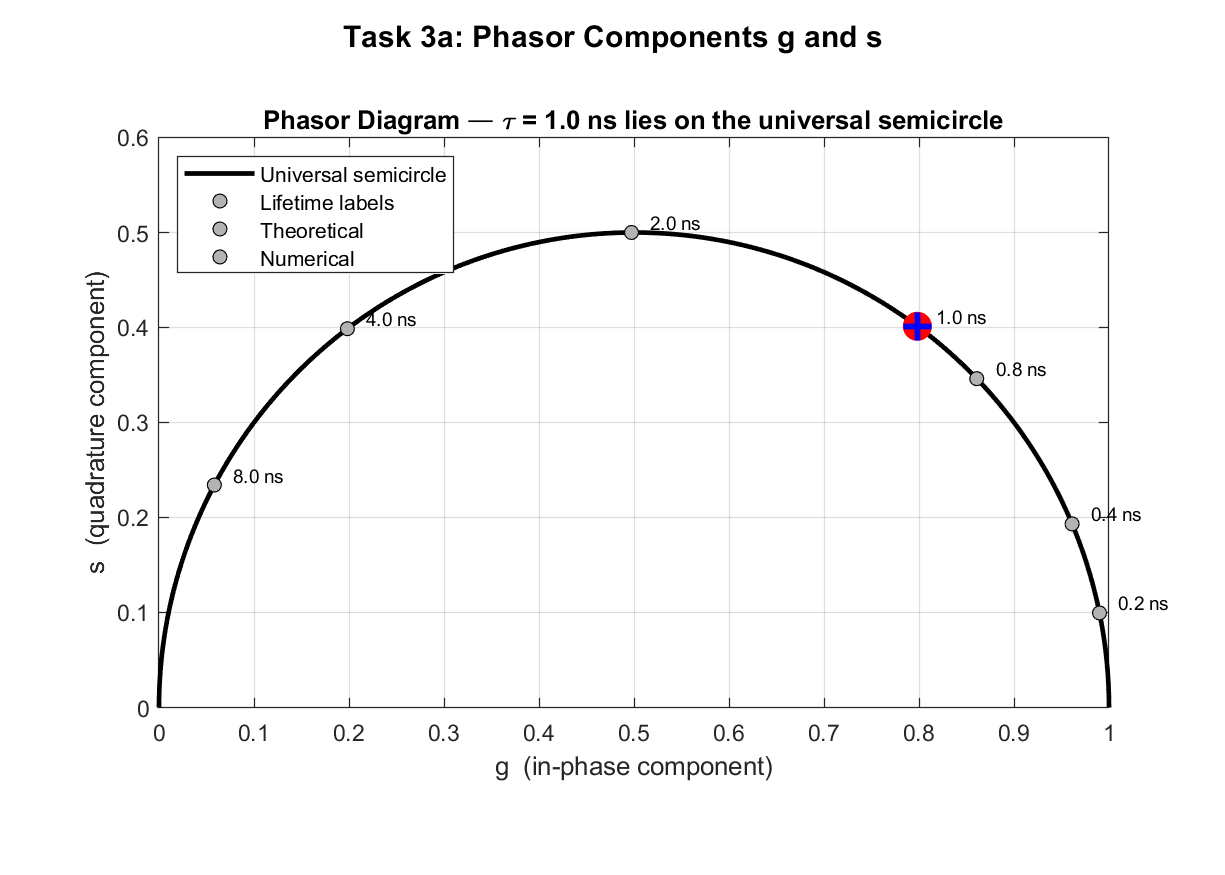
\includegraphics[width=\linewidth]{figs/fig_phasor_diagram.png}
    \caption{Phasor diagram for $\tau = 1\,\text{ns}$ at
             $f_L = 80\,\text{MHz}$.
             Theoretical (red circle) and numerical (blue cross) both
             lie on the universal semicircle (black).
             Shorter lifetimes appear near $(g,s) = (1,0)$; longer
             lifetimes approach $(0,0)$.}
    \label{fig:phasor_diagram}
\end{figure}

\subsubsection{Fluorescence Lifetime Image}

Fig.~\ref{fig:lifetime_image} shows the per-pixel lifetime map of the
breast cancer cell dataset, color-scaled to $[0,3]\,\text{ns}$.
The image reveals substantial spatial heterogeneity consistent with
co-existing free and protein-bound NAD(P)H populations.
Regions with shorter lifetimes ($\tau \lesssim 0.5\,\text{ns}$, blue)
are consistent with \emph{free} NAD(P)H, which has a reported solution
lifetime of $0.3$--$0.5\,\text{ns}$~\cite{Datta2020}.
Longer-lifetime regions ($\tau \sim 1$--$3\,\text{ns}$, yellow--red)
correspond to \emph{protein-bound} NAD(P)H, whose lifetime is elongated
by restricted molecular motion~\cite{Sorrells2021}.
This spatial distribution of free-to-bound NAD(P)H reflects the local
metabolic activity of the cells: a shift toward bound NAD(P)H indicates
oxidative phosphorylation, while predominantly free NAD(P)H is
characteristic of the aerobic glycolysis (Warburg effect) common in
cancer cells.

\begin{figure}[!t]
    \centering
    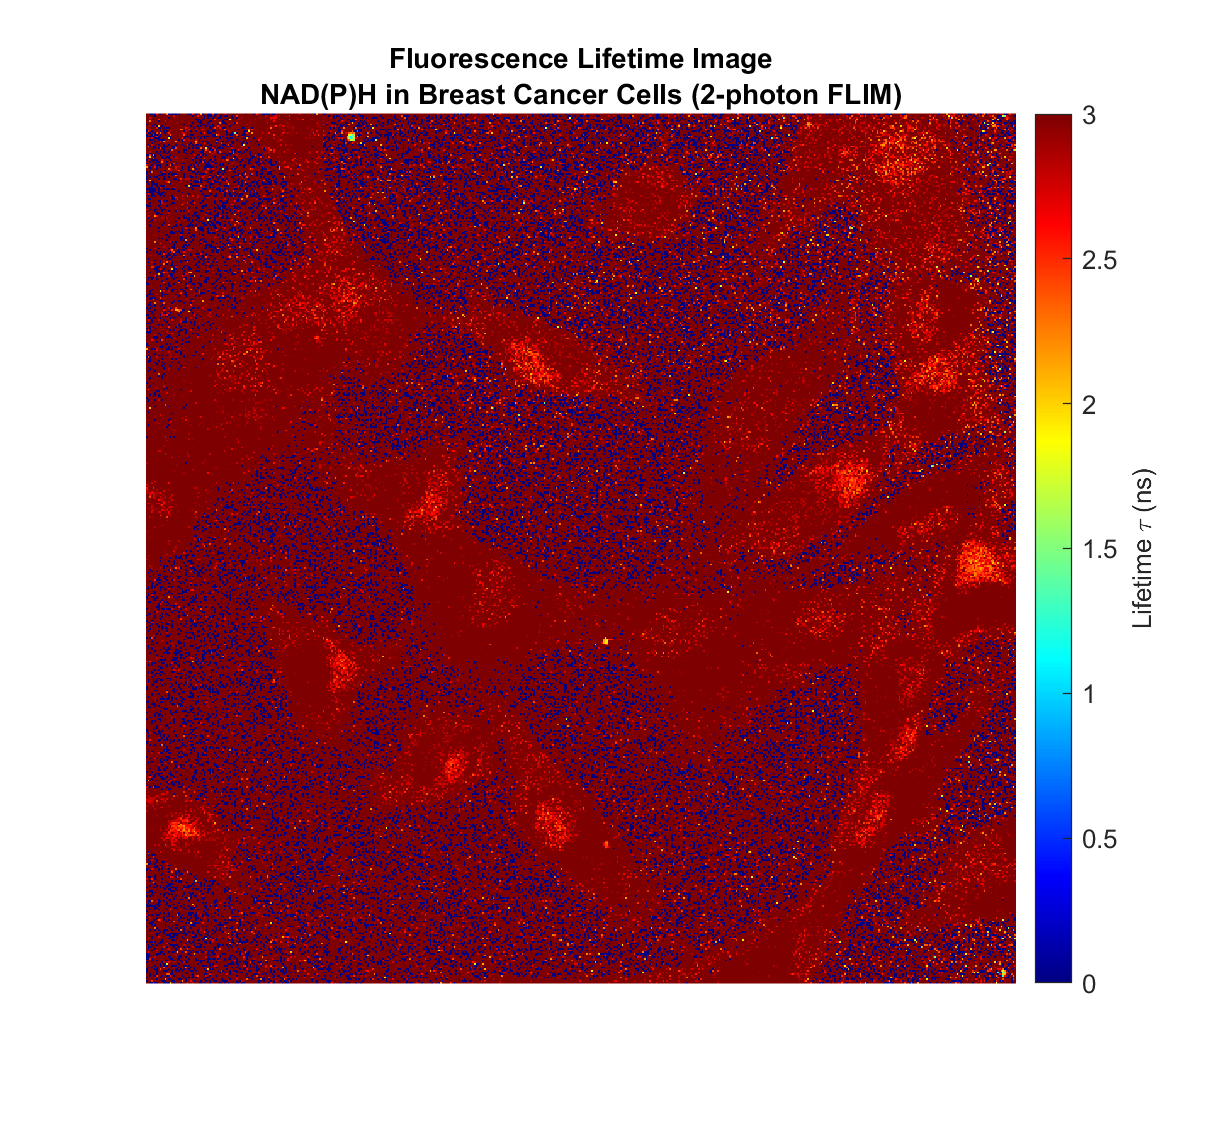
\includegraphics[width=\linewidth]{figs/fig_lifetime_image.png}
    \caption{Per-pixel fluorescence lifetime map of NAD(P)H in breast
             cancer cells ($512\times512$ pixels).
             Color scale: $0$--$3\,\text{ns}$ (\texttt{jet} colormap).
             Blue: free NAD(P)H; yellow--red: protein-bound NAD(P)H.}
    \label{fig:lifetime_image}
\end{figure}

\subsubsection{Phasor Plot}

Fig.~\ref{fig:phasor_plot} shows the pixelwise phasor plot as a
log-scaled 2D density histogram overlaid with the universal semicircle.
Several features are apparent.
The pixel cloud lies \emph{inside} the semicircle, indicating that most
pixels contain a mixture of free and bound NAD(P)H; for a two-species
mixture, the phasor sits on the chord connecting the two pure-species
points inside the semicircle.
A high-density cluster near $(g \approx 0.95,\,s \approx 0.10)$
corresponds to free NAD(P)H ($\tau \approx 0.3$--$0.5\,\text{ns}$),
while a lower-density tail toward $(g \approx 0.65,\,s \approx 0.38)$
indicates protein-bound NAD(P)H ($\tau \approx 1$--$2\,\text{ns}$).
A small fraction of pixels fall just outside the semicircle due to
shot noise and the finite integration window bias for long lifetimes.

Phasor analysis provides two key practical advantages over
pixel-by-pixel exponential fitting.
First, it is non-iterative---requiring only two dot products per pixel
(Eqs.~\eqref{eq:g_discrete}--\eqref{eq:s_discrete})---and scales
trivially to megapixel images.
Second, the 2D phasor plot can be used as a segmentation tool: drawing
a region-of-interest on the phasor and back-projecting to the image
isolates pixels with a specific biochemical state without any additional
fitting.
One limitation is that the single-frequency phasor yields a
\emph{phase-weighted mean} lifetime rather than resolving individual
components; separating two species would require multi-harmonic analysis
or global fitting~\cite{Gadella1993}.

\begin{figure}[!t]
    \centering
    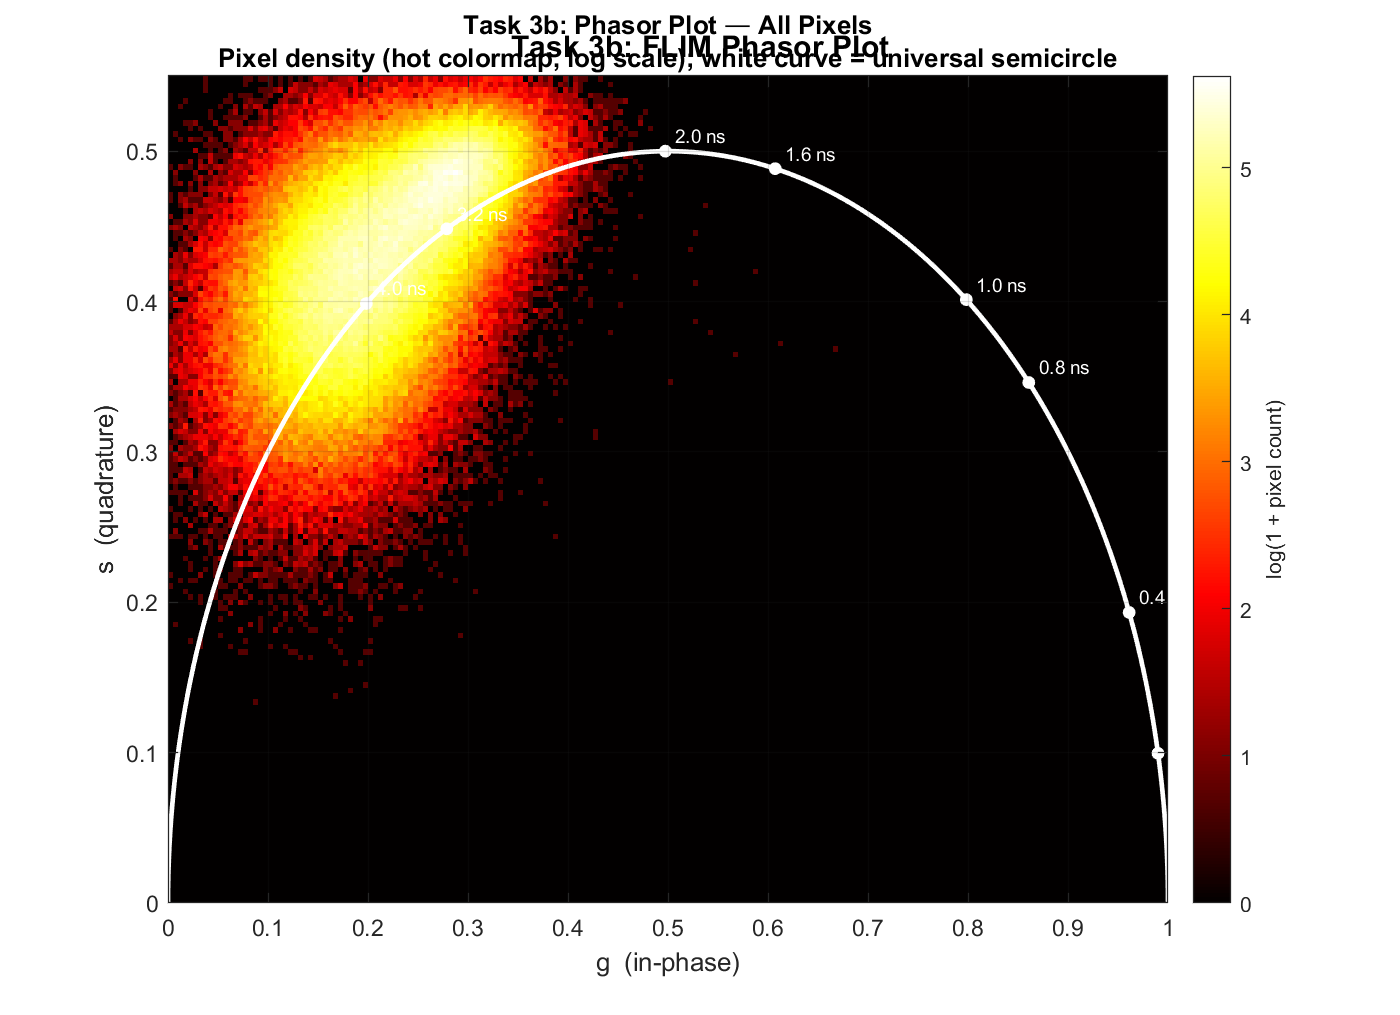
\includegraphics[width=\linewidth]{figs/fig_phasor_plot.png}
    \caption{Pixelwise phasor plot (log-density, \texttt{hot} colormap).
             White curve: universal semicircle; white circles: reference
             lifetimes at $0.2$--$3.2\,\text{ns}$.
             The cloud lies inside the semicircle, consistent with
             multi-exponential (mixed free/bound) NAD(P)H.}
    \label{fig:phasor_plot}
\end{figure}



\section{Conclusion}

This study applied LTI system theory to three distinct fluorescence
lifetime measurement scenarios, each illustrating a different
relationship between physical signal processing and biological
information extraction.
In the time domain, the convolution chain faithfully reproduced the
pulsed-FLIM signal; the detector IRF was identified as the dominant
source of lifetime overestimation when $\sigma_t$ is comparable to
$\tau$, requiring more complex curve fitting methods to recover the true decay.
Heterodyne detection resolved the 80\,MHz
fluorescence signal being undetectable by a 100\,kHz ADC by mixing
to a 1\,kHz beat frequency, both the phase shift
$\Delta\varphi = -\arctan(\omega_L\tau)$ and modulation depth
$M = 1/\sqrt{1+(\omega_L\tau)^2}$ were preserved, independently
recovering $\tau = 1\,\text{ns}$ with high accuracy.
Phasor analysis unified the frequency-domain perspective into a
two-coordinate representation that scales efficiently to imaging
data; applied to real NAD(P)H TCSPC measurements, it produced a
lifetime map distinguishing free from protein-bound populations and a
phasor plot whose interior cloud directly encodes the metabolic state of individual cells
without a single iterative fit.
Together, the three tasks demonstrate that the mathematics of
convolution, Fourier analysis, and inner-product projections are not
merely abstract tools but the direct computational substrate of
modern biomedical imaging.

\begin{thebibliography}{00}

\bibitem{Datta2020}
R. Datta, T. M. Heaster, J. T. Sharick, A. A. Gillette, and M. C. Skala,
``Fluorescence lifetime imaging microscopy: fundamentals and advances in
instrumentation, analysis, and applications,''
\textit{J. Biomed. Opt.}, vol.~25, no.~7, pp.~1--43, May 2020.

\bibitem{Gadella1993}
T. W. J. Gadella, T. M. Jovin, and R. M. Clegg,
``Fluorescence lifetime imaging microscopy: pixel-by-pixel analysis of
time-resolved fluorescence images,''
\textit{Biophys. Chem.}, vol.~48, no.~2, pp.~221--239, 1993.

\bibitem{Digman2008}
M. A. Digman, V. R. Caiolfa, M. Zamai, and E. Gratton,
``The phasor approach to fluorescence lifetime imaging analysis,''
\textit{Biophys. J.}, vol.~94, no.~2, pp.~L14--L16, Jan. 2008.

\bibitem{Sorrells2021}
J. E. Sorrells, E. M. Martin, E. Aksamitiene \textit{et al.},
``Label-free characterization of single extracellular vesicles using
two-photon fluorescence lifetime imaging microscopy of {NAD(P)H},''
\textit{Sci. Rep.}, vol.~11, p.~3308, 2021.

\end{thebibliography}

\clearpage
\onecolumn
\appendices


\end{document}
